%\setchapterpreamble[u]{
%\dictum[Johann Wolfgang von Goethe]{Es ist nicht genug, zu wissen, man muß auch anwenden; es ist nicht genug, zu wollen, man muß auch tun. \dots}}
\section{Use Cases}\label{kap:Use_Cases} 
% Funktionale Anforderungen

Dieses Kapitel beschreibt mögliche Use Cases die sich aus ISO 29002-31 ergeben. 

Die Query-Code-Beispiele sind gekürzt, d.h. es werden beispielsweise referenzierte Schemata-Namen nicht aufgeführt. 

\begin{figure}[htbp]
	\centering
		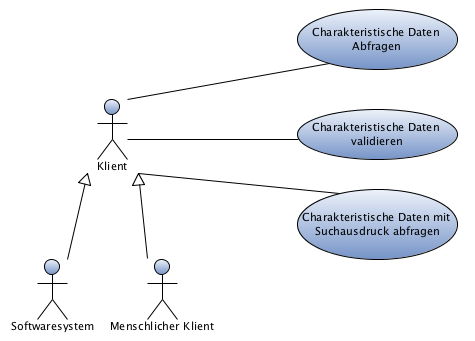
\includegraphics[width=0.75\textwidth]{images/usecases_plib.png}
	\caption{Use Case Übersicht}
	\label{fig:usecaseuebersicht}
\end{figure}

\subsection{Akteure}
Bei der Implementierung geht es um eine generische Schnittstelle. In den nachfolgenden Anwendungsfällen wird vom Akteur \enquote{Klient} gesprochen. Der Klient ist allgemein ein Nutzer der Schnittstelle, sei es als menschlicher Akteur welcher über eine Bedienerinterface die Schnittstelle benutzt oder eine direkte Maschinennutzung.    

%TODO Use Case Diagram

\subsection{Use Case Beschreibungen}

\subsubsection{Alle Charakteristische Daten eines Produkts abfragen}

{\small

\begin{description}
     \item[use case] Charakteristische Daten abfragen
     \item[  actors]~\\
     Klient
     \item[  precondition]~\\
     Der Klient verwendet einen gültigen Identifier.
     \item[  main flow]~\\
     Der Klient gibt einen Identifier (IRDI\footnote{International Registration Data Identifier}) einer Klasse von Elementen ein und sendet eine Anfrage ab. Die Anfrage wird auf Gültigkeit überprüft. Als Antwort bekommt er ein oder mehrere Datensätze von Elementen \footnote{Item, ISO 29002-10 Kapitel 5.3.2} mit den entsprechenden charakteristischen Daten \footnote{property\_values, ISO 29002-10 Kapitel 5.2.4}  des Elementes mit dem übergebenen Identifier zurück.
     \item[  postcondition]~\\
     Alle Daten aller Elemente der gewählten Klassen des Identifiers wurden zurückgegeben.    
     \item[  alternative flow] Properties auswählen ~\\
     Zusammen mit dem Identifier übergibt der Klient einen oder mehrere Property-Identifier und sendet diese erweiterte Anfrage ab.    
     \item[  postcondition]~\\
     Die mittels Property-Identifier ausgewählten Daten aller Elemente der gewählten Klassen wurden zurückgegeben.    
     \item[end] Charakteristische Daten abfragen
\end{description}

~\\

} %end small

\paragraph{Beispiel}

Ein Schraubendreher könnte folgendermaßen in einer Produktdatenbank repräsentiert werden:

\begin{description}\label{lab:schraubendreher}
\item[Klassen-Identifier] 0173-1\#01-AAA352\#4 
\item[Länge] 300mm
\item[Typ] Kreuz
\item[Spannungsfest] ja
\end{description}

Korrekterweise müssten anstatt der Attribute wie Länge oder Typ ebenfalls ein Identifier stehen. Die Benamungen sind hier zur besseren Lesbarkeit aufgelöst. 

Um nun alle Eigenschaften (Properties), wie Länge, Typ und Spannungsfest zu erhalten muss folgende Abfrage gesendet werden: 
\textbf{"Gib mir alle Items und alle Properties der Klasse mit dem Identifier 0173-1\#01-AAA352\#4 (Schraubendreher)".}
Das Ergebnis ist ein Item mit allen Attributen (Properties) der gewünschten Klassen und gegebenenfalls vorhandenen Unterklassen. In unserem Falle genau die oben angegebenen Werte.

Die XML-Abfrage sieht wie folgt aus:

\begin{lstlisting}[caption=Query Beispiel - Daten abfragen, language=XML, label=UseCaseDatenabfragen]
<?xml version="1.0" encoding="UTF-8"?>
<qy:query xsi:schemaLocation="...query query.xsd" xmlns:xsi="http://www.w3.org/2001/XMLSchema-instance" xmlns:cat="...catalogue" xmlns:val="...value" xmlns:qy="...query" xmlns:bas="...basic">
	<qy:class_ref>0173-1#01-AAA352#4</qy:class_ref>
</qy:query>
\end{lstlisting}

Eine Abfrage, welche die Properties der Klasse auswählt die zurückgeliefert werden sollen könnte lauten: 
\textbf{"Gib mir alle Items und die Properties Länge und Typ der Klasse mit dem Identifier 0173-1\#01-AAA352\#4 (Schraubendreher)".}
Das Ergebnis ist ein Item mit den gewünschten Attributen (Properties). 

Die XML-Abfrage:
\begin{lstlisting}[caption=Query Beispiel - Daten abfragen mit Propertyeinschränkung, language=XML, label=lst:UseCaseDatenabfragenProperty]

<?xml version="1.0" encoding="UTF-8"?>
<qy:query xsi:schemaLocation="...query query.xsd" xmlns:xsi="http://www.w3.org/2001/XMLSchema-instance" xmlns:cat="...catalogue" xmlns:val="...value" xmlns:qy="...query" xmlns:bas="...basic">
	<qy:class_ref>0173-1#01-AAA352#4</qy:class_ref>
	
	<!-- typ und laenge -->
	<qy:property_ref>0173-1#01-BBB111#1 0173-1#01-BBB222#1</qy:property_ref> 
	
</qy:query>
\end{lstlisting}

Listing \ref{lst:UseCaseDatenabfragenProperty} beinhaltet ein XML-Attribut property\_ref. Das wird mit gewünschten Property Identifier gefüllt, welche mit Leerzeichen getrennt werden. 

\subsubsection{Charakteristische Daten eines Produkts validieren}

{\small

\begin{description}
     \item[use case] Charakteristische Daten validieren
     \item[  actors]~\\
     Klient
     \item[  precondition]~\\
     Der Klient verwendet einen gültigen Identifier sowie auf den Identifier passende Daten..
     \item[  main flow]~\\
     Der Klient gibt einen Identifier eines Elementes (Klasse) ein. Zusätzlich übermittelt er zu diesem bekanntem Element Eigenschaften dieser Instanz des Elements und sendet eine Anfrage ab. Die Anfrage wird auf Gültigkeit überprüft. Als Antwort bekommt er ein oder mehrere Datensätze von Elementen mit den entsprechenden charakteristischen Daten zurück, auf welche die übergebenen Eigenschaften am besten zutreffen. 
     \item[  postcondition]~\\
     Alle Daten aller Elemente der gewählten Klassen des Identifiers werden zurückgegeben. Dies ermöglicht dem Klienten eine Validierung der ihm bereits bekannten Daten über ein Element. 
     \item[end] Charakteristische Daten validieren
\end{description}

~\\

} %end small

\paragraph{Beispiel}

In diesem Anwendungsfall verfügen wir bereits über Elemente/Wertenpaare einer bestimmten Klasse, z.B. eben jenen Schraubendreher

\textbf{"Ich habe hier ein mir bekanntes Item mit bestimmten Eigenschaften (Properties), Länge=300mm. Gib mir alle Items und alle Properties der Klasse mit dem Identifier 0173-1\#01-AAA352\#4 (Kreuzschraube) welche die mitgelieferten Eigenschaften haben".}
Das Ergebnis sind Items mit allen Properties der angegebenen Klasse, welche über die übergebenen Eigenschaften (Properties) verfügen. In unserem Fall vervollständigen wir unsere Properties mit den weiteren Properties "Typ" und "Spannungsfest".

Die XML-Abfrage sieht so aus:

\begin{lstlisting}[caption=Query Beispiel - Daten abfragen, language=XML, label=UseCaseDatenabfragen]
<?xml version="1.0" encoding="UTF-8"?>
<qy:query xsi:schemaLocation="...query query.xsd" xmlns:xsi="http://www.w3.org/2001/XMLSchema-instance" xmlns:cat="...catalogue" xmlns:val="...value" xmlns:qy="...query" xmlns:bas="...basic">
	<cat:item class_ref="0173-1#01-AAA352#4..">
		<cat:property_value property_ref="0173-1#01-BBB111#1">
			<val:integer_value></val:integer_value>
		</cat:property_value>
	</cat:item>
</qy:query>
\end{lstlisting}

\subsubsection{Chrarakteristische Daten mittels Suchausdruck abfragen }

{\small

\begin{description}
     \item[use case] Charakteristische Daten mit Suchausdruck abfragen
     \item[  actors]~\\
     Klient
     \item[  precondition]~\\
     Der Klient verwendet einen gültigen Identifier.
     \item[  main flow]~\\
     Der Klient gibt einen Identifier eines Elementes (Klasse) ein. Ferner übergibt er ein oder mehrere bekannte Property Identifier sowie passend dazu Werte zur Sucheinschränkung. 
     \item[  postcondition]~\\
     Alle Elemente auf jene diese Einschränkung der übergebenen Werte zutrifft wurden zurückgegeben. 
     \item[end] Charakteristische Daten mit Suchausdruck abfragen
\end{description}

~\\

} %end small

\paragraph{Beispiel}

Wir nehmen das Schraubendreher Beispiel aus \ref{lab:schraubendreher} zur Hand, und möchten eine Abfrage absenden, welche von der Klasse Schraubendreher alle Items erhalten soll die eine Länge zwischen 200 und 300 mm haben. 

Um nun alle Eigenschaften (Properties), wie Länge, Typ und Spannungsfest zu erhalten muss folgende Abfrage gesendet werden: 
\textbf{"Gib mir alle Items und alle Properties der Klasse mit dem Identifier 0173-1\#01-AAA352\#4 (Kreuzschraube)".}
Das Ergebnis ist ein Item mit allen Attributen (Properties) der gewünschten Klassen und gegebenenfalls vorhandenen Unterklassen. In unserem Falle genau die oben angegebenen Werte.

Die XML-Abfrage sieht so aus:

\begin{lstlisting}[caption=Query Beispiel - Daten abfragen, language=XML, label=UseCaseDatenabfragen]
<?xml version="1.0" encoding="UTF-8"?>
<qy:query xsi:schemaLocation="...query query.xsd" xmlns:xsi="http://www.w3.org/2001/XMLSchema-instance" xmlns:cat="...catalogue" xmlns:val="...value" xmlns:qy="...query" xmlns:bas="...basic">
	<qy:class_ref>0173-1#01-AAA352#4</qy:class_ref>
	<qy:characteristic_data_query_expression>
		<qy:range>
			<qy:property_reference property_ref="0173-1#01-BBB111#1"/>
			<qy:min_value>200</qy:min_value>
			<qy:max_value>300</qy:max_value>
			<qy:is_inclusive>true</qy:is_inclusive>
		</qy:range>
	</qy:characteristic_data_query_expression>
</qy:query>
\end{lstlisting}


%\section{Automatisierte Benutzerebene}
%Der Unterschied zur manuellen Benutzerebene ist der, dass hierbei automatisiert Daten angefragt und übermittelt werden. Es findet keine Mensch zu %Maschine Kommunikation statt sondern eine Maschine zu Maschine Kommunikation. 
%Ziel der automatisierten Anfragen ist das Abgleichen oder Validieren von Massendaten eines (Teil)-Katalogs. 

%\begin{description}
%\item[Alle Klassen abfragen] Der Klient sendet eine Anfrage und erhält alle vorhandene Klassen (ohne Items).
%\item[Items einer Klasse abgleichen] Der Klient möchte seine Daten abgleichen und fragt alle Items einer Klasse ab.  
%\item[Items einer Klasse validieren] Der Klient möchte seine Daten validieren und fragt alle Items einer Klasse ab.
%\end{description}